\newcommand{\object}[3]{
\begin{tabular}[h!]{| p{7cm} |}
	\hline
	\begin{center}\textbf{#1}\end{center} \\ \hline
	\begin{mylist} #2 \end{mylist} \\ \hline
	\begin{mylist} #3 \end{mylist} \\ \hline

\end{tabular}
}

\newenvironment{mylist}{
	\begin{enumerate}[label=+]
}{
	\end{enumerate}
}

\section{Object Models}

\begin{figure}[h!]
\begin{center}
	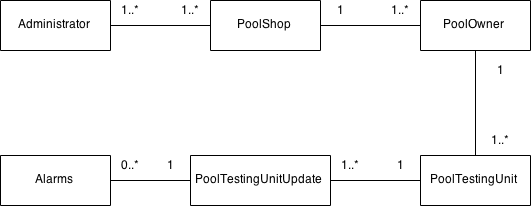
\includegraphics[width=15cm]{images/ObjectRelations}
	\caption{relationships between the main classes in the system}
\end{center}
\end{figure}

\par
There can be multiple administrators in the SPACS system that manage all the PoolShopAdmin. Each PoolOwner can only be registered at one PoolShopAdmin, and each PoolTestingUnit can only be linked to one PoolOwner. The Administrator, PoolShopAdmin and PoolOwner objects all contain information about a single person.
\par
The above figure shows the basics of how the different objects interact, and not the helper classes that ensure these links are done correctly. More information on how these classes interact can be found below.

\subsection{Objects}
\subsubsection{User}
\par
User is the class that all users of the system will fall under. It ensures a minimum amount of information is collected about each user and will implement all the basic instructions needed for interacting with the objects. The level property allows the user object to do this. Authentication information is stored in the Authentication object to minimize the ability to leak sensitive information, such as passwords from it.

\object{User(object)}
{
	\item id
	\item title
	\item name
	\item address 
	\item email\_address
	\item phone\_number
	\item mobile\_number
	\item level
}
{
	\item
}

\object{Authentication(object)}
{
	\item id
	\item username
	\item password
}
{
	\item
}

\subsubsection{Administrator, PoolShop and PoolOwner}
\par
These are all extensions of the User object and will implement any extra methods that they do not inherit. Pythonic code doesn't use setter and getter functions, but still allows the properties to have validation on them.

\object{Administrator(User)}
{
	\item 
}
{
	\item
}

\object{PoolShop(User)}
{
	\item pool\_owners
}
{
	\item 
}

\object{PoolOwner(User)}
{
	\item pool\_testing\_units
}
{
	\item
}

\subsubsection{ShopOwnerLink}
\par
ShopOwnerLink stores the link between a PoolShopAdmin and a PoolOwner, ensuring that  a PoolShopAdmin can only see pools that they manage.

\object{ShopOwnerLink(object)}
{
	\item pool\_shop\_admin\_id
	\item pool\_owner\_id
}
{
	\item
}

\subsubsection{PoolTestingUnit}
\par
Pool Testing Units are mostly passive users of the system and have the sole role of providing information to the system. They are closely linked to their PoolOwner. Again, due to the way python works this object should have no methods.

\object{PoolTestingUnit(object)}
{
	\item ptu\_id
	\item owner\_id
	\item length
	\item width
	\item depth
	\item volume
	\item above\_ground
	\item material
						
}
{
	\item
}

\subsubsection{PoolTestingUnitUpdate}
\par
PoolTestingUnitUpdate objects store all the information from the records that the pool testing units send.

\object{PoolTestingUnitUpdate(object)}
{
	\item report\_id
	\item ptu\_id
	\item datetime
	\item pH
	\item chlorine\_level
	\item chlorinator\_status
	\item total\_alkalinity
	\item temperature
	\item water\_hardness
	\item water\_level
	\item datetime\_last\_filter
	\item alarms
}
{
	\item
}

\subsubsection{Alarm}
\par
Alarm objects store alarms set off when a PoolTestingUnit sends a PoolTestingUnitUpdate.

\object{PoolTestingUnitUpdate(object)}
{
	\item alarm\_id
	\item report\_id
	\item reason
	\item value
	\item expected
}
{
	\item
}